\begin{tikzpicture}[
	every axis/.style={
		%grid=major,
		%grid style={dotted},
		ybar stacked,
		%ylabel={"Time [s]"},
		%ymode=log,
		%ymin=0,ymax=15,
		y tick label style={
			font=\footnotesize
		},
		x tick label style={
			% add some negative yshift to move ticklabels down
			yshift=-2mm,
			rotate=45,
			anchor=east,
			font=\scriptsize
		},
		%x axis line style = { opacity = 0 }, 
		%y axis line style = { opacity = 0 },
		tickwidth = 0pt,
		width=\textwidth,
		height=0.3\textheight,
		% symbolic coords have numerical distance of 1
		% so with the following line you get a tick at every symbolic coord
		xtick distance=1,
		symbolic x coords={CESM-ATM,ISABEL,NYX,SCALE-LETKF,QMCPACK,Miranda,S3D,EXAFEL},
		bar width=4pt
	},
	]
	\pgfplotsset{
		% define a new style used for the plot used to add labels
		% 2 args means it takes two mandatory arguments, so must be used as
		% labelplot={first arg}{second arg}
		labelplot/.style 2 args={
			% forget plot means it doesn't affect cycle lists or legends
			forget plot,
			% #1 is first argument, the text used in the nodes near coords
			nodes near coords=#1,
			% #2 is second argument, a length that should be the same as the bar shift for the axis
			every node near coord/.style={below,font=\tiny,xshift=#2}
		}
	}
	
	\begin{axis}[bar shift=-12pt,grid=major,grid style={dotted},ylabel={Time [s]},ymin=0,ymax=15,yticklabels={0,5,10,15},ytick={0,5,10,15}] % tlib
		\addplot [labelplot={1st}{-12pt}] coordinates {(CESM-ATM,0) (ISABEL,0) (NYX,0) (SCALE-LETKF,0) (QMCPACK,0) (Miranda,0) (S3D,0) (EXAFEL,0)};
		\addplot+[fill=blue!30!white] coordinates { (CESM-ATM,0.632) (ISABEL,0.086) (NYX,0.186) (SCALE-LETKF,1.406) (QMCPACK,0.009) (Miranda,0.043) (S3D,0.328) (EXAFEL,0.179) };
		\addplot+[fill=red!30!white] coordinates { (CESM-ATM,0.006) (ISABEL,0.026) (NYX,0.177) (SCALE-LETKF,0.117) (QMCPACK,0.018) (Miranda,0.034) (S3D,0.284) (EXAFEL,2.474) };
		\addplot+[fill=yellow!30!white] coordinates { (CESM-ATM,0.017) (ISABEL,0.034) (NYX,0.311) (SCALE-LETKF,0.204) (QMCPACK,0.014) (Miranda,0.042) (S3D,0.323) (EXAFEL,1.084) };
		\addplot+[fill=green!30!white] coordinates { (CESM-ATM,0.017) (ISABEL,0.160) (NYX,2.846) (SCALE-LETKF,1.096) (QMCPACK,0.011) (Miranda,0.610) (S3D,3.277) (EXAFEL,1.278) };
	\end{axis}

	\begin{axis}[bar shift=-6pt, xticklabels={},ymin=0,ymax=15,yticklabels={}] % tuckermpi
		\addplot [labelplot={2nd}{-6pt}]coordinates {(CESM-ATM,0) (ISABEL,0) (NYX,0) (SCALE-LETKF,0) (QMCPACK,0) (Miranda,0) (S3D,0) (EXAFEL,0)};
		\addplot+[fill=blue!30!white] coordinates { (CESM-ATM,0.378) (ISABEL,0.083) (NYX,0.181) (SCALE-LETKF,1.092) (QMCPACK,0.010) (Miranda,0.043) (S3D,0.352) (EXAFEL,0.172) };
		\addplot+[fill=red!30!white] coordinates { (CESM-ATM,0.050) (ISABEL,0.136) (NYX,0.504) (SCALE-LETKF,0.633) (QMCPACK,0.312) (Miranda,0.157) (S3D,0.631) (EXAFEL,8.191) };
		\addplot+[fill=yellow!30!white] coordinates { (CESM-ATM,0.017) (ISABEL,0.036) (NYX,0.401) (SCALE-LETKF,0.237) (QMCPACK,0.020) (Miranda,0.091) (S3D,0.417) (EXAFEL,1.706) };
		\addplot+[fill=green!30!white] coordinates { (CESM-ATM,0.013) (ISABEL,0.110) (NYX,2.601) (SCALE-LETKF,0.618) (QMCPACK,0.011) (Miranda,0.350) (S3D,2.920) (EXAFEL,1.400) };
	\end{axis}
	
	\begin{axis}[bar shift=0pt,xticklabels={},ymin=0,ymax=15,yticklabels={}] % tblis
		\addplot [labelplot={3rd}{0pt}] coordinates {(CESM-ATM,0)      (ISABEL,0)      (NYX,0)      (SCALE-LETKF,0)      (QMCPACK,0) (Miranda,0) (S3D,0) (EXAFEL,0)};
		\addplot+[fill=blue!30!white] coordinates { (CESM-ATM,1.017) (ISABEL,0.152) (NYX,0.293) (SCALE-LETKF,2.063) (QMCPACK,0.021) (Miranda,0.065) (S3D,0.456) (EXAFEL,0.269) };
		\addplot+[fill=red!30!white] coordinates { (CESM-ATM,0.013) (ISABEL,0.031) (NYX,0.221) (SCALE-LETKF,0.144) (QMCPACK,0.018) (Miranda,0.035) (S3D,0.372) (EXAFEL,4.831) };
		\addplot+[fill=yellow!30!white] coordinates { (CESM-ATM,0.019) (ISABEL,0.033) (NYX,0.369) (SCALE-LETKF,0.164) (QMCPACK,0.019) (Miranda,0.056) (S3D,0.503) (EXAFEL,1.776) };
		\addplot+[fill=green!30!white] coordinates { (CESM-ATM,0.017) (ISABEL,0.240) (NYX,6.184) (SCALE-LETKF,1.044) (QMCPACK,0.013) (Miranda,0.953) (S3D,4.936) (EXAFEL,1.010) };
	\end{axis}

	\begin{axis}[bar shift=6pt,xticklabels={},ymin=0,ymax=15,yticklabels={}] % tcl
		\addplot [labelplot={4th}{6pt}] coordinates {(CESM-ATM,0)      (ISABEL,0)      (NYX,0)      (SCALE-LETKF,0)      (QMCPACK,0) (Miranda,0) (S3D,0) (EXAFEL,0)};
		\addplot+[fill=blue!30!white] coordinates { (CESM-ATM,0.600) (ISABEL,0.130) (NYX,0.197) (SCALE-LETKF,1.539) (QMCPACK,0.017) (Miranda,0.045) (S3D,0.330) (EXAFEL,0.203) };
		\addplot+[fill=red!30!white] coordinates { (CESM-ATM,0.024) (ISABEL,0.062) (NYX,0.626) (SCALE-LETKF,0.417) (QMCPACK,0.055) (Miranda,0.142) (S3D,0.615) (EXAFEL,0.970) };
		\addplot+[fill=yellow!30!white] coordinates { (CESM-ATM,0.017) (ISABEL,0.062) (NYX,0.501) (SCALE-LETKF,0.311) (QMCPACK,0.039) (Miranda,0.123) (S3D,0.604) (EXAFEL,1.393) };
		\addplot+[fill=green!30!white] coordinates { (CESM-ATM,0.017) (ISABEL,0.195) (NYX,4.203) (SCALE-LETKF,1.275) (QMCPACK,0.012) (Miranda,0.803) (S3D,3.881) (EXAFEL,2.322) };
	\end{axis}
	
	\begin{axis}[bar shift=12pt,xticklabels={},ymin=0,ymax=15,yticklabels={}] % eigen
		\addplot [labelplot={5th}{12pt}] coordinates {(CESM-ATM,0)      (ISABEL,0)      (NYX,0)      (SCALE-LETKF,0)      (QMCPACK,0) (Miranda,0) (S3D,0) (EXAFEL,0)};	
		\addplot+[fill=blue!30!white] coordinates { (CESM-ATM,2.782) (ISABEL,0.652) (NYX,1.221) (SCALE-LETKF,3.720) (QMCPACK,0.084) (Miranda,0.359) (S3D,1.848) (EXAFEL,0.538) };
		\addplot+[fill=red!30!white] coordinates { (CESM-ATM,0.654) (ISABEL,0.408) (NYX,1.036) (SCALE-LETKF,4.903) (QMCPACK,0.071) (Miranda,0.271) (S3D,1.717) (EXAFEL,0.970) };
		\addplot+[fill=yellow!30!white] coordinates { (CESM-ATM,1.304) (ISABEL,0.406) (NYX,1.029) (SCALE-LETKF,4.886) (QMCPACK,0.081) (Miranda,0.269) (S3D,1.707) (EXAFEL,1.393) };
		\addplot+[fill=green!30!white] coordinates { (CESM-ATM,1.299) (ISABEL,0.193) (NYX,0.651) (SCALE-LETKF,1.067) (QMCPACK,0.130) (Miranda,0.213) (S3D,0.886) (EXAFEL,2.322) };
	\end{axis}

	\begin{axis}[bar shift=18pt,xticklabels={},ymin=0,ymax=15,yticklabels={}] % torch
		\addplot [labelplot={5th}{18pt}] coordinates {(CESM-ATM,0)      (ISABEL,0)      (NYX,0)      (SCALE-LETKF,0)      (QMCPACK,0) (Miranda,0) (S3D,0) (EXAFEL,0)};
		\addplot+[fill=blue!30!white] coordinates { (CESM-ATM,0.620) (ISABEL,0.117) (NYX,0.194) (SCALE-LETKF,1.403) (QMCPACK,0.015) (Miranda,0.050) (S3D,0.327) (EXAFEL,0.127) };
		\addplot+[fill=red!30!white] coordinates { (CESM-ATM,0.061) (ISABEL,0.127) (NYX,0.399) (SCALE-LETKF,0.442) (QMCPACK,0.069) (Miranda,0.160) (S3D,0.616) (EXAFEL,3.919) };
		\addplot+[fill=yellow!30!white] coordinates { (CESM-ATM,0.014) (ISABEL,0.115) (NYX,0.387) (SCALE-LETKF,0.393) (QMCPACK,0.067) (Miranda,0.166) (S3D,0.585) (EXAFEL,1.491) };
		\addplot+[fill=green!30!white] coordinates { (CESM-ATM,0.013) (ISABEL,0.106) (NYX,2.875) (SCALE-LETKF,0.600) (QMCPACK,0.011) (Miranda,0.381) (S3D,2.949) (EXAFEL,1.135) };
	\end{axis}	
	
	%\begin{axis}[bar shift=6pt,xticklabels={},ymin=0,ymax=15,yticklabels={}]
	%	\addplot [labelplot={4rd}{6pt}] coordinates {(CESM-ATM,0)     (ISABEL,0)     (NYX,0)      (SCALE-LETKF,0)      (QMCPACK,0) (Miranda,0) (S3D,0) (EXAFEL,0)};
	%	\addplot+[fill=blue!30!white] coordinates { (CESM-ATM,9.233) (ISABEL,2.957) (NYX,5.293) (SCALE-LETKF,35.131) (QMCPACK,0.276) (Miranda,1.402) (S3D,8.675) (EXAFEL,2.351) };
	%	\addplot+[fill=red!30!white] coordinates { (CESM-ATM,0.131) (ISABEL,0.681) (NYX,4.997) (SCALE-LETKF,3.554) (QMCPACK,0.296) (Miranda,0.912) (S3D,8.931) (EXAFEL,71.757) };
	%	\addplot+[fill=yellow!30!white] coordinates { (CESM-ATM,0.099) (ISABEL,0.666) (NYX,4.926) (SCALE-LETKF,3.544) (QMCPACK,0.265) (Miranda,0.904) (S3D,8.883) (EXAFEL,30.443) };
	%	\addplot+[fill=green!30!white] coordinates { (CESM-ATM,0.100) (ISABEL,2.195) (NYX,50.854) (SCALE-LETKF,12.268) (QMCPACK,0.206) (Miranda,6.696) (S3D,49.788) (EXAFEL,27.820) };
	%\end{axis}


\end{tikzpicture}
